\documentclass[border=5pt]{standalone}
%%%<
\usepackage{verbatim}
%%%>
\usepackage{pgfplots}
\pgfplotsset{width=7cm,compat=1.8}
\usepgfplotslibrary{ternary}
\begin{comment}
:Title: Density map in ternary diagram
:Tags: 2D;Color maps;Ternary diagrams
:Author: eject
:Slug: ternary-diagram-density-map

This is a ternary diagram where each point does has a fourth value, besides
the three that are the coordinates. Instead of stating this fourth value as a
node next to each plotted point, the points should be coloured according to
their value.

This code was posted by eject on TeX.SE.
\end{comment}
\renewcommand*{\familydefault}{\sfdefault}
\usepackage{sfmath}
\begin{document}
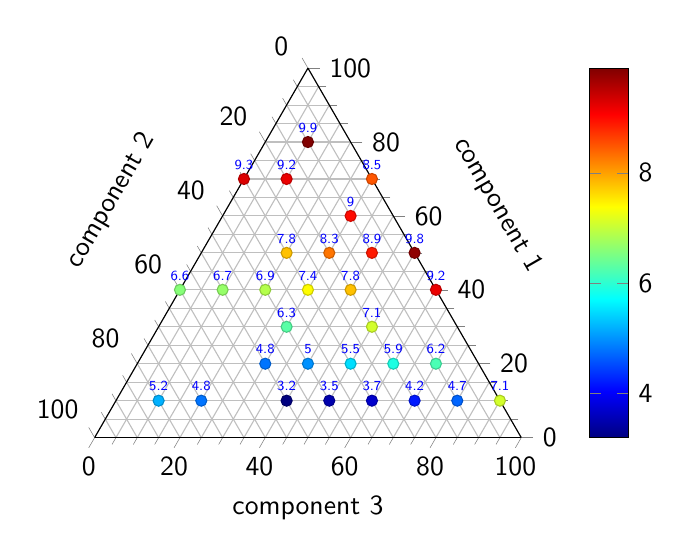
\begin{tikzpicture}
  \begin{ternaryaxis}[colorbar, colormap/jet,
    xmin = 0,
    xmax = 100,
    ymin = 0,
    ymax = 100,
    zmin = 0,
    zmax = 100, 
    xlabel = component 1,
    ylabel = component 2,
    zlabel = component 3,
    grid   = both,
    label style    = {sloped},
    minor tick num = 3,
  ]
  \addplot3+[only marks, 
    point meta=\thisrow{myvalue}, %  uses ’point meta’ as color data.
    nodes near coords*={\tiny{\pgfmathprintnumber\myvalue}}, %does what it says
    visualization depends on={\thisrow{myvalue} \as \myvalue} %defines visualization dependency
  ] table {
    x       y       z       myvalue
    10      0       90      7.1
    40      0       60      9.2
    50      0       50      9.8
    70      0       30      8.5
    20      30      50      5.5
    20      20      40      5
    20      50      30      4.8
    30      40      30      6.3
    30      20      50      7.1
    40      20      40      7.8
    40      30      30      7.4
    40      40      20      6.9
    40      50      10      6.7
    10      10      80      4.7
    10      20      70      4.2
    10      30      60      3.7
    10      40      50      3.5
    10      50      40      3.2
    10      70      20      4.8
    10      80      10      5.2
    50      30      20      7.8
    50      20      30      8.3
    60      10      30      9
    70      20      10      9.2
    80      10      10      9.9
    20      10      70      6.2
    40      60      0       6.6
    70      30      0       9.3
    50      10      40      8.9
    20      20      60      5.9
  };
  \end{ternaryaxis}
\end{tikzpicture}
\end{document}
